\documentclass[conference]{IEEEtran}

\usepackage[noadjust]{cite}
\usepackage{subfig}
\usepackage{balance}
\usepackage{verbatim}
\usepackage{flushend}
\usepackage{hyperref}


% *** GRAPHICS RELATED PACKAGES ***
%
\ifCLASSINFOpdf
  \usepackage[pdftex]{graphicx}
  % declare the path(s) where your graphic files are
  % \graphicspath{{../pdf/}{../jpeg/}}
  % and their extensions so you won't have to specify these with
  % every instance of \includegraphics
  % \DeclareGraphicsExtensions{.pdf,.jpeg,.png}
\else
  % or other class option (dvipsone, dvipdf, if not using dvips). graphicx
  % will default to the driver specified in the system graphics.cfg if no
  % driver is specified.
  % \usepackage[dvips]{graphicx}
  % declare the path(s) where your graphic files are
  % \graphicspath{{../eps/}}
  % and their extensions so you won't have to specify these with
  % every instance of \includegraphics
  % \DeclareGraphicsExtensions{.eps}
\fi

\usepackage{algorithm}
\usepackage[noend]{algorithmic}

\usepackage{multirow}
\usepackage{amsmath}
\usepackage{xcolor}

\renewcommand{\algorithmicrequire}{\textbf{Input:}}
\renewcommand{\algorithmicensure}{\textbf{Output:}}

% correct bad hyphenation here
\hyphenation{op-tical net-works semi-conduc-tor}



\begin{document}

\title{Hot Deployment with Dependency Reconstruction}

\author{\IEEEauthorblockN{Haicheng Li, Chun Cao,  Ping Yu}
\IEEEauthorblockA{State Key Lab for Novel Software Technology, Nanjing University, Nanjing, China\\
Dept. of Computer Science and Technology, Nanjing University, Nanjing, China\\
lhc\_happy@sina.cn, \{caochun, yuping\}@nju.edu.cn}
}

% make the title area
\maketitle


\begin{abstract}
Hot deployment is a typical feature in mainstream application servers. But current application servers treat each module as a standalone application and may fail if a module with dependencies against other ones is partially updated with hot deploying. The reason lies in that those module dependencies are not respected in current application servers. Direct countermeasures that manage dependencies in application servers are actually inefficient or even infeasible. So in this paper, we propose an approach that automatically constructs the module dependencies with class loading mechanism which furthermore helps to reconstruct the modular application respecting the dependencies upon hot deploying. Experiments show that our technology of hot deployment can ensure partial update of the modular applications correctly and efficiently.
\end{abstract}

\begin{IEEEkeywords}
Hot deployment; Dependency reconstruction; Class loading.
\end{IEEEkeywords}


\IEEEpeerreviewmaketitle


\section{Introduction\label{sec:introduction}}

Nowadays application servers\cite{app_server} provide platforms for enterprise applications to be deployed, operated and maintained. They usually contain comprehensive services, such as clustering, security and transaction management, et. al, so that developers can focus on the business logic. As one of those sophisticated services, hot deployment enables the server to put applications into production without restarting the server itself. By hot deployment, the existing application can be upgraded in this fashion as well.

The technology of hot deployment highly improves the efficiency and flexibility of the application servers.
It becomes one of the typical features of mainstream application server products, such as JBoss\cite{jboss} and WebLogic\cite{weblogic}, which play a significant role in the development of enterprise applications. By the philosophy of design of the application servers, the units to be deployed, in packages (or modules) of ear/war/jar, are standalone applications, which means they are closed and self-contained. This implicit assumption does not prohibit the developers to build the applications that span multiple packages with internal dependencies. Applications in this case can still work as long as the referencing across different deployment units are supported. As a matter of fact, the unit deploying mechanisms built in the application servers like JBoss do make this happen with appropriate class loader designed. Application servers ensure that modules are deployed after the deployment of modules which it depends on. The dependencies are constructed in the context of deployment unit during the first time deployment.

Applications in multiple packages, which are called as \emph{modular applications}, are common when they are developed by different individuals collaboratively or assembled with third-party libraries that are already packed independently. They still work fine on application servers until some portion of the application is about to be hot deployed  with the new versions. As the application server treats the packages as isolated ones, it ignores the existence of potential relationships among the modules. Failures may happen because the original dependencies between the portion to be hot deployed and the rest of the application are broken, which makes the whole application down.

To solve the problem, the dependencies need to be reconstructed. Intuitively, this can be done manually. The developer should have the knowledge of dependent configuration among the application modules and be aware of the affection scope of the redeployment. Then they can redeploy the dependent ones by hand. However, this requires human intervention which can be strenuous and even error-prone, especially for large-scale applications. Alternatively, they can also redeploy all the modules for that application. But it not only is unnecessary, but also causes the state of unaffected part to be destructed, such as the data storage module which is hardly updated. 

In this paper, we introduce a general approach to enable the correct hot deployment respecting the dependencies among modules. The dependencies which are constructed with class loaders for the modules and upon the dependent modules can be calculated. Their hot deployment can be triggered when depended modules are hot deployed. In order to update flexibly and efficiently, we can obtain and manage dependencies from the dynamic way with lazy reconstruction during hot deployment, so that the dependent modules only update their class loaders and they don't need to do anything else except class loading in the process of redeployment. Experiments show that the problems of calling failure can be solved through this technology and the efficiency of application servers is improved.

The rest of this paper is organized as follow. 
Section \ref{sec:background} reviews the hot deployment mechanisms and analyzes the reasons of failures based on the hot deployment mechanisms. 
Section \ref{sec:reconstructionAS} describes dependency reconstruction in application servers, which is a common approach to solve dependency lost.
And Section \ref{sec:reconstructionCL} presents a more effective approach of dependency reconstruction with class loaders.
We give the evaluations in Section \ref{sec:evaluation} and Section \ref{sec:relatedwork} is the related work.
Lastly in Section \ref{sec:conclusion}, we conclude this paper and discuss future work.



\section{Background\label{sec:background}}
In this section, the hot deployment mechanisms of current application servers are investigated. We also analyze the causes of failures in hot deploying the modular applications.

\subsection{Hot Deployment}

Hot deployment built in mainstream application servers enables applications on the servers to be published, updated or withdrawn without restarting the servers. This feature is based on the class loading mechanism beyond the standard class loaders\cite{standard_cl} in Java system. Conceptually, each module to be deployed, has its own class loader as a standalone application instead of sharing one with other modules so that the standalone application in that module can be independently operated. All the effective module class loaders are organized together (in a chain or pool) so that they can find each other and delegate each other to load classes and resources which enables the mutual referring and sharing among the modules. When a module is hot deployed, the corresponding module class loader will be removed and a new one will be created to load the new version of the module. In this way, application servers complete hot deployment of applications\cite{module_cl}.

\begin{figure}[ht]
\centering
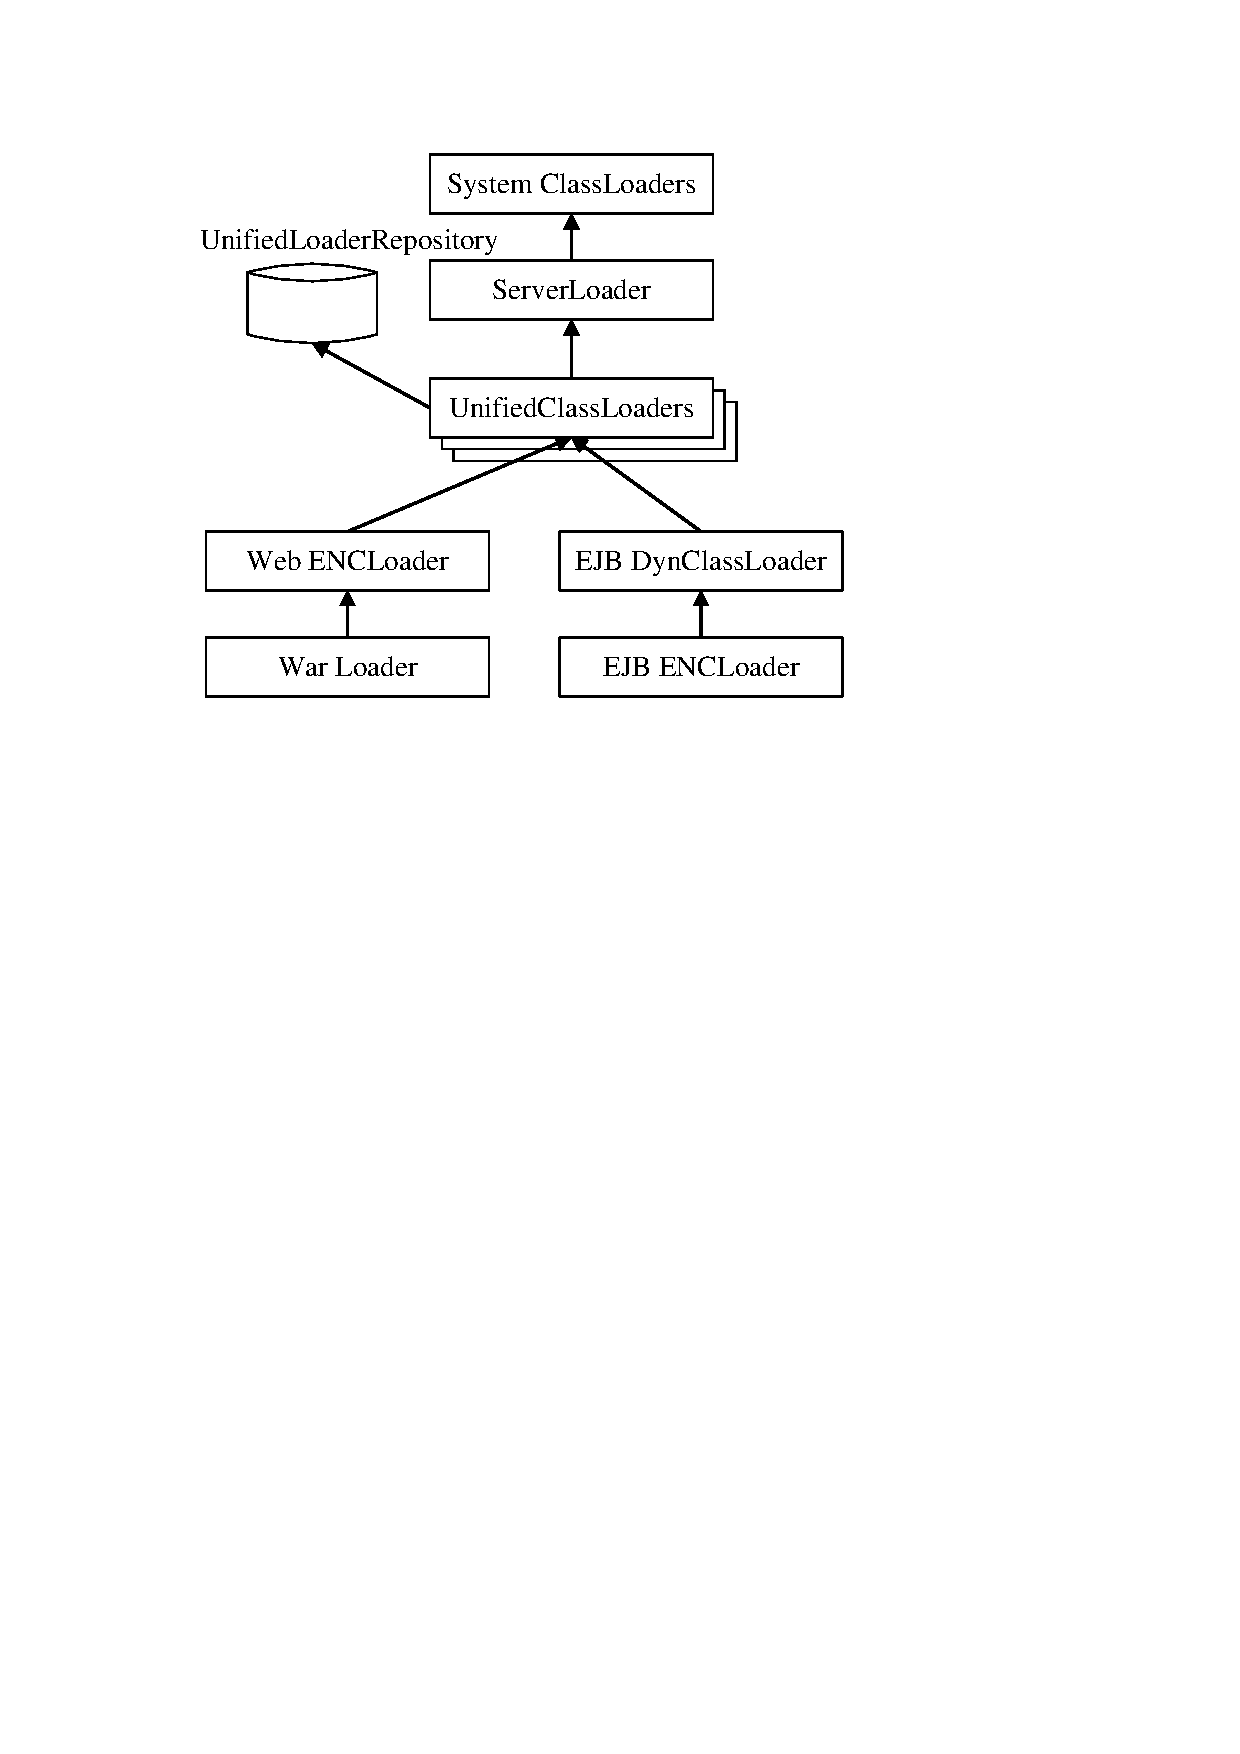
\includegraphics[width=3.0in]{JBossClassLoader.pdf}
\caption{class loader architecture in JBoss}
\label{fig:jboss_class_loader}
\end{figure}

Fig. \ref{fig:jboss_class_loader} shows an illustrative architecture of class loading in JBoss and other application servers adopt the similar design. As for JBoss, \emph{ServerLoader} is responsible to load JBoss server itself. For applications of different types, including EARs, JARs, WARs, etc., seen by the deployment scanner, the server applies various loaders, including \emph{EJB ENCLoader} and \emph{Web ENCLoader}, to load classes respectively. Furthermore, each class loader delegates the \emph{UnifiedClassLoader} to manage the classes loaded in a repository\cite{jboss_class_loader}. Fig. \ref{fig:example} shows two EJBs\cite{EJB} packed in JARs. Each EJB contains only one class here for simplicity. Class \emph{ComputeBean} in Computer.jar is a session bean for dividing calculation. Class \emph{ValidatorBean} is another session bean that verifies whether a number is zero or not. If these two modules are deployed in JBoss, two \emph{EJB ENCLoader} instances are responsible for loading the classes and they delegate two \emph{UnifiedClassLoader} instances to load classes. So each \emph{UnifiedClassLoader} instance serves the corresponding module as its module class loader.


\begin{figure}[ht]
\centering
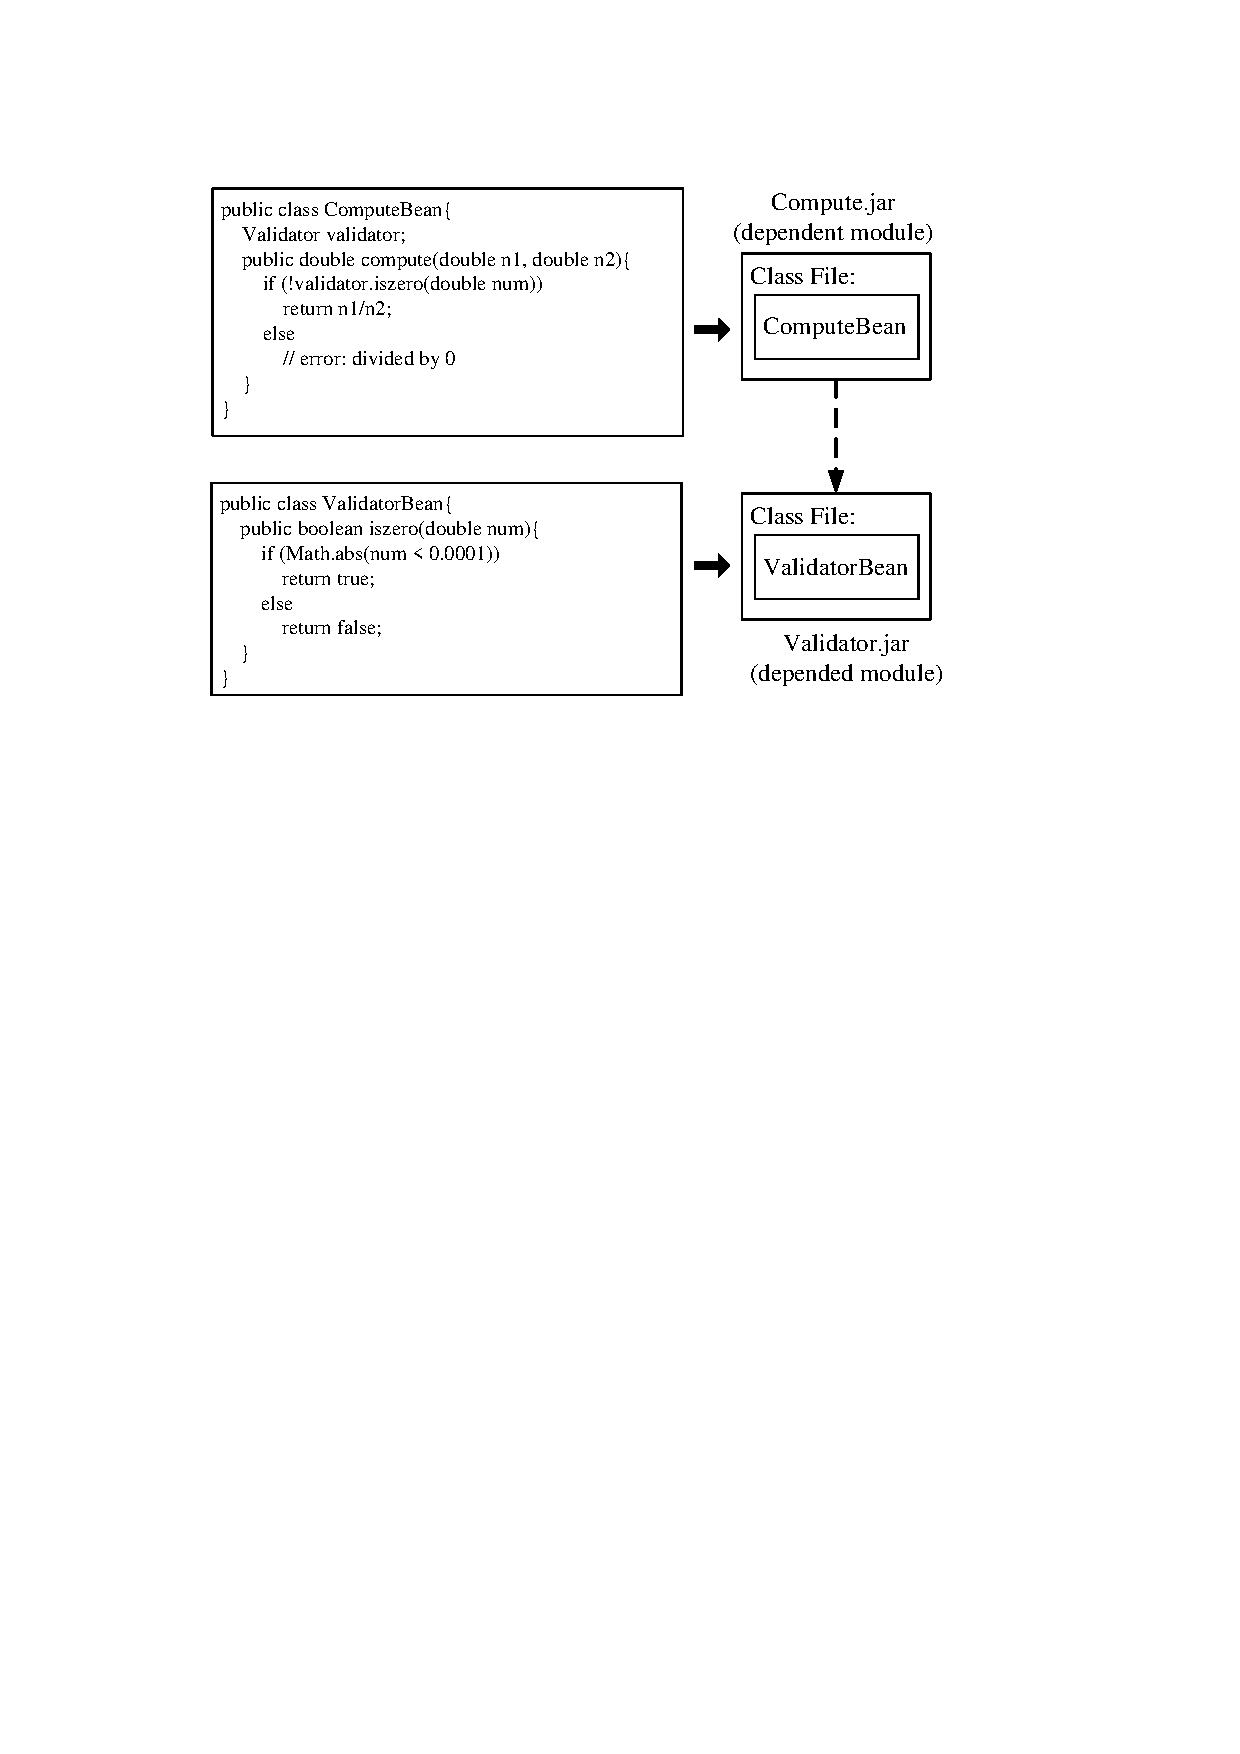
\includegraphics[width=3.5in]{ExampleEJB.pdf}
\caption{a modular application for dividing calculation}
\label{fig:example}
\end{figure}


\subsection{Hot Deployment Failures Caused by Module Dependency}

\begin{figure}[ht]
\centering
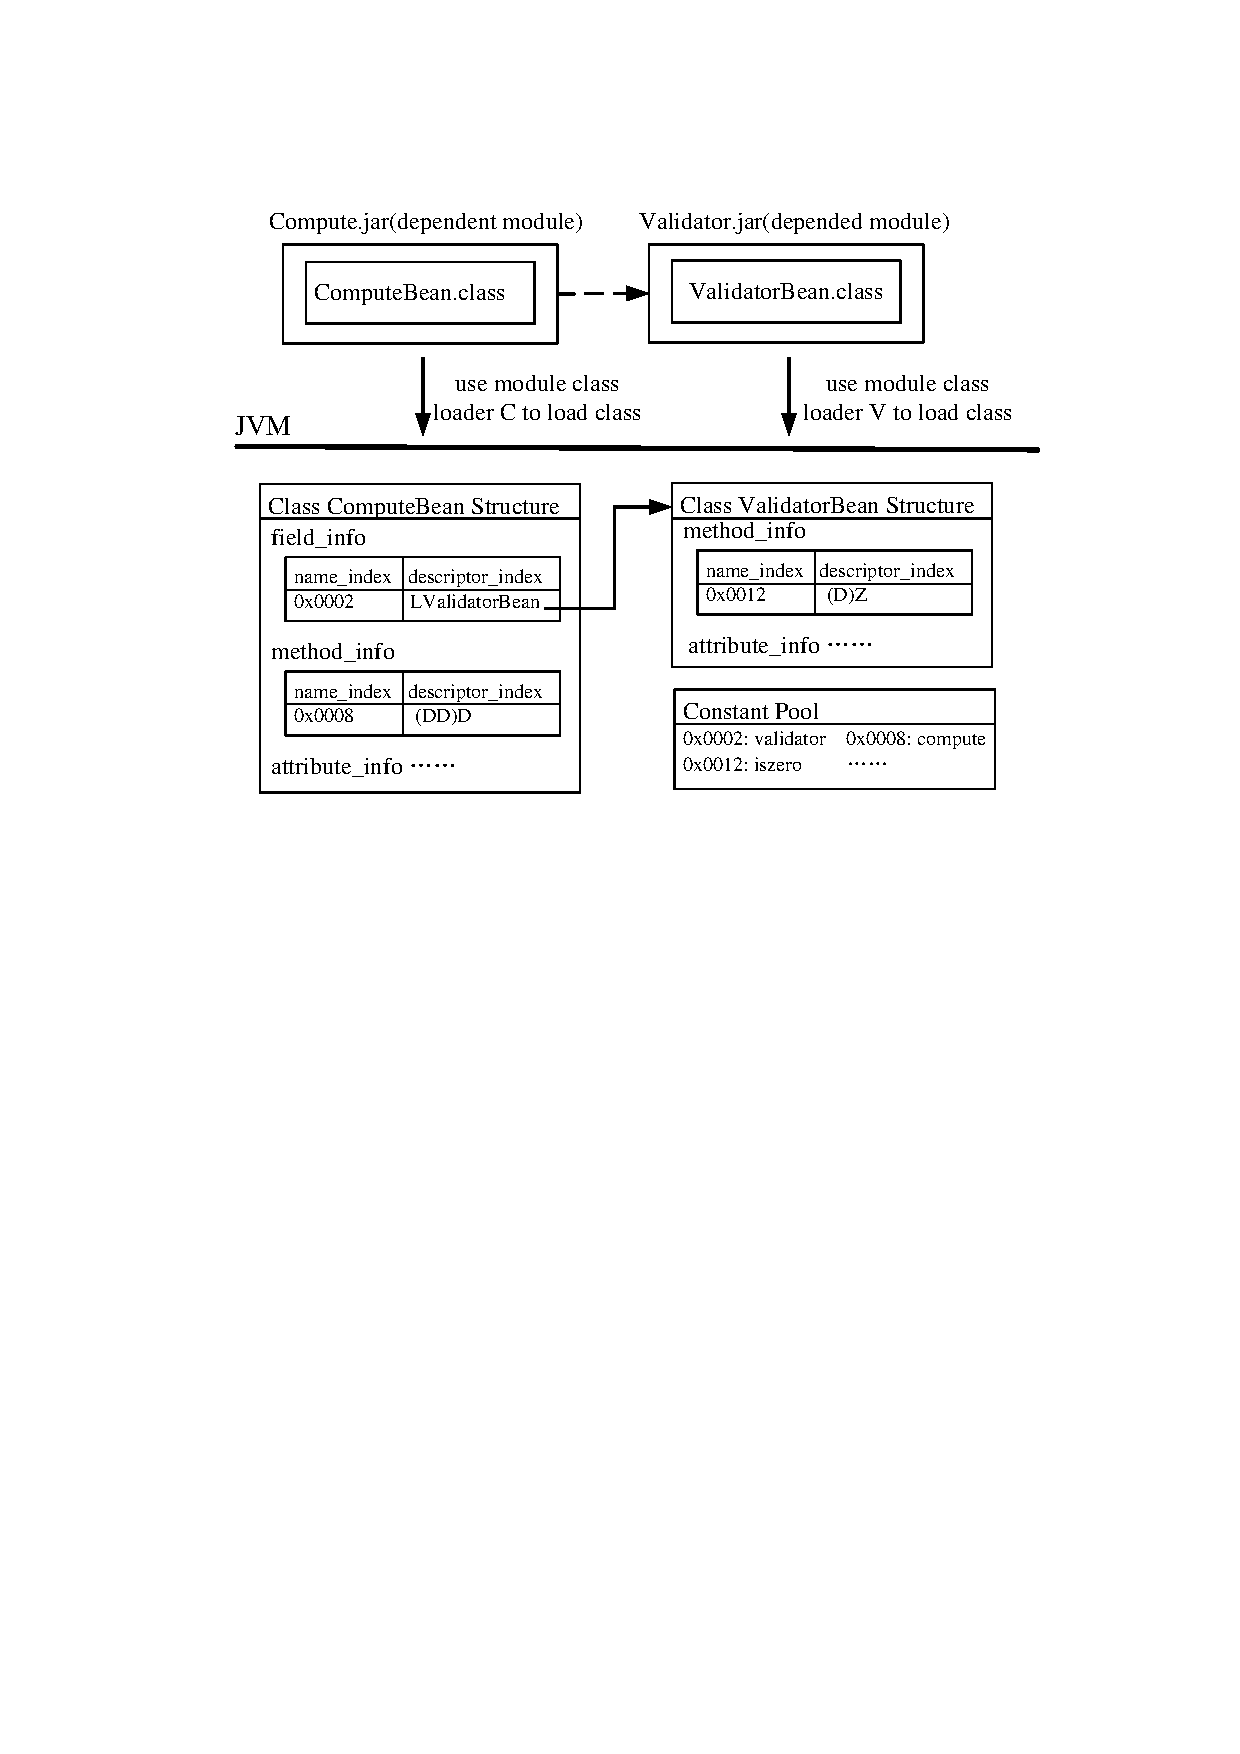
\includegraphics[width=3.5in]{ExampleJVM.pdf}
\caption{a modular application and loading details}
\label{fig:example_jvm}
\end{figure}

The modules in the above example actually have an internal dependency between them as class \emph{ComputeBean} uses \emph{iszero} method of class \emph{ValidatorBean} to verify whether the divisor is zero or not by referring the latter class. Such a reference takes effect because while the classes are loaded into the JVM\cite{jvm}, the information of the classes are resolved by their module class loaders and stored in their own class structure tables in the virtual machine. As for the reference against \emph{ValidatorBean}, the \emph{field\_info} table of \emph{ComputeBean} stores the address of the class structure of \emph{ValidatorBean}, as shown in Fig. \ref{fig:example_jvm}. In short, we can find the field name \emph{validator} and field type \emph{ValidatorBean} from the index in the \emph{field\_info} of class structure of \emph{ComputeBean}. 
The \emph{name\_index} points to an entry in the constant pool and the \emph{descriptor\_index} points to the referenced class structure if this variable is a reference type\cite{jvm_book}. 

At the first time of deployment, the dependency can be captured by the server because each module must be check whether it meets dependencies before deployment. Depended modules must be deployed before dependent ones, so that applications can be operated normally after module deployment and class loading. However, if the depended module is hot deployed again later, calling failures may occur after running the whole application. For example, if the class \emph{ValidatorBean} raises its floating point precision from 0.0001 to 0.00001 and the new packed JAR file Validator.jar is dropped into the server, calling class \emph{ComputeBean} will then throw an exception. 

It is due to the fact that according to the JVM specification\cite{jvm_specification}, a class loader cannot load a class more than once, which means the original class loader cannot be used to load the new version of class \emph{ValidatorBean}. So the server will simply destroy the existing class loader for Validator.jar and create a new one for the lately deployed one while Compute.jar remains untouched. The class structure of class \emph{ValidatorBean} in JVM is recreated and maintained in a new place in the memory. In this case, the original reference becomes invalid. The dependency between the two modules is broken and it consequently causes a failure.


\section{Dependency Reconstruction in Application Servers\label{sec:reconstructionAS}}

To support hot deployment of modular applications, the key is to reconstruct the broken dependencies. An intuitive approach is to enable the application server to find the mutual dependencies among the modules and refresh the dependent ones to build the broken dependencies. The dependencies among modules can be explicitly stated by the application developers. Developers can provide the profiles of modules to describe their dependencies. The dependencies will be collected as soon as the modules are deployed in application servers. Fig. \ref{fig:example_abc} is a modular application with three modules A, B and C. Module A depends on module B and module C, which is described as a profile A-JAR.xml. When deploying them at the first time, servers can create dependency mapping table by these profiles. If module B is hot deployed later, servers will realize module A depends on module B. Then module A must be redeployed and its module class loader must be updated after the hot deployment of module B. In this way, the broken dependencies are reconstructed simply and the calling failure problems are solved.

\begin{figure}[ht]
\centering
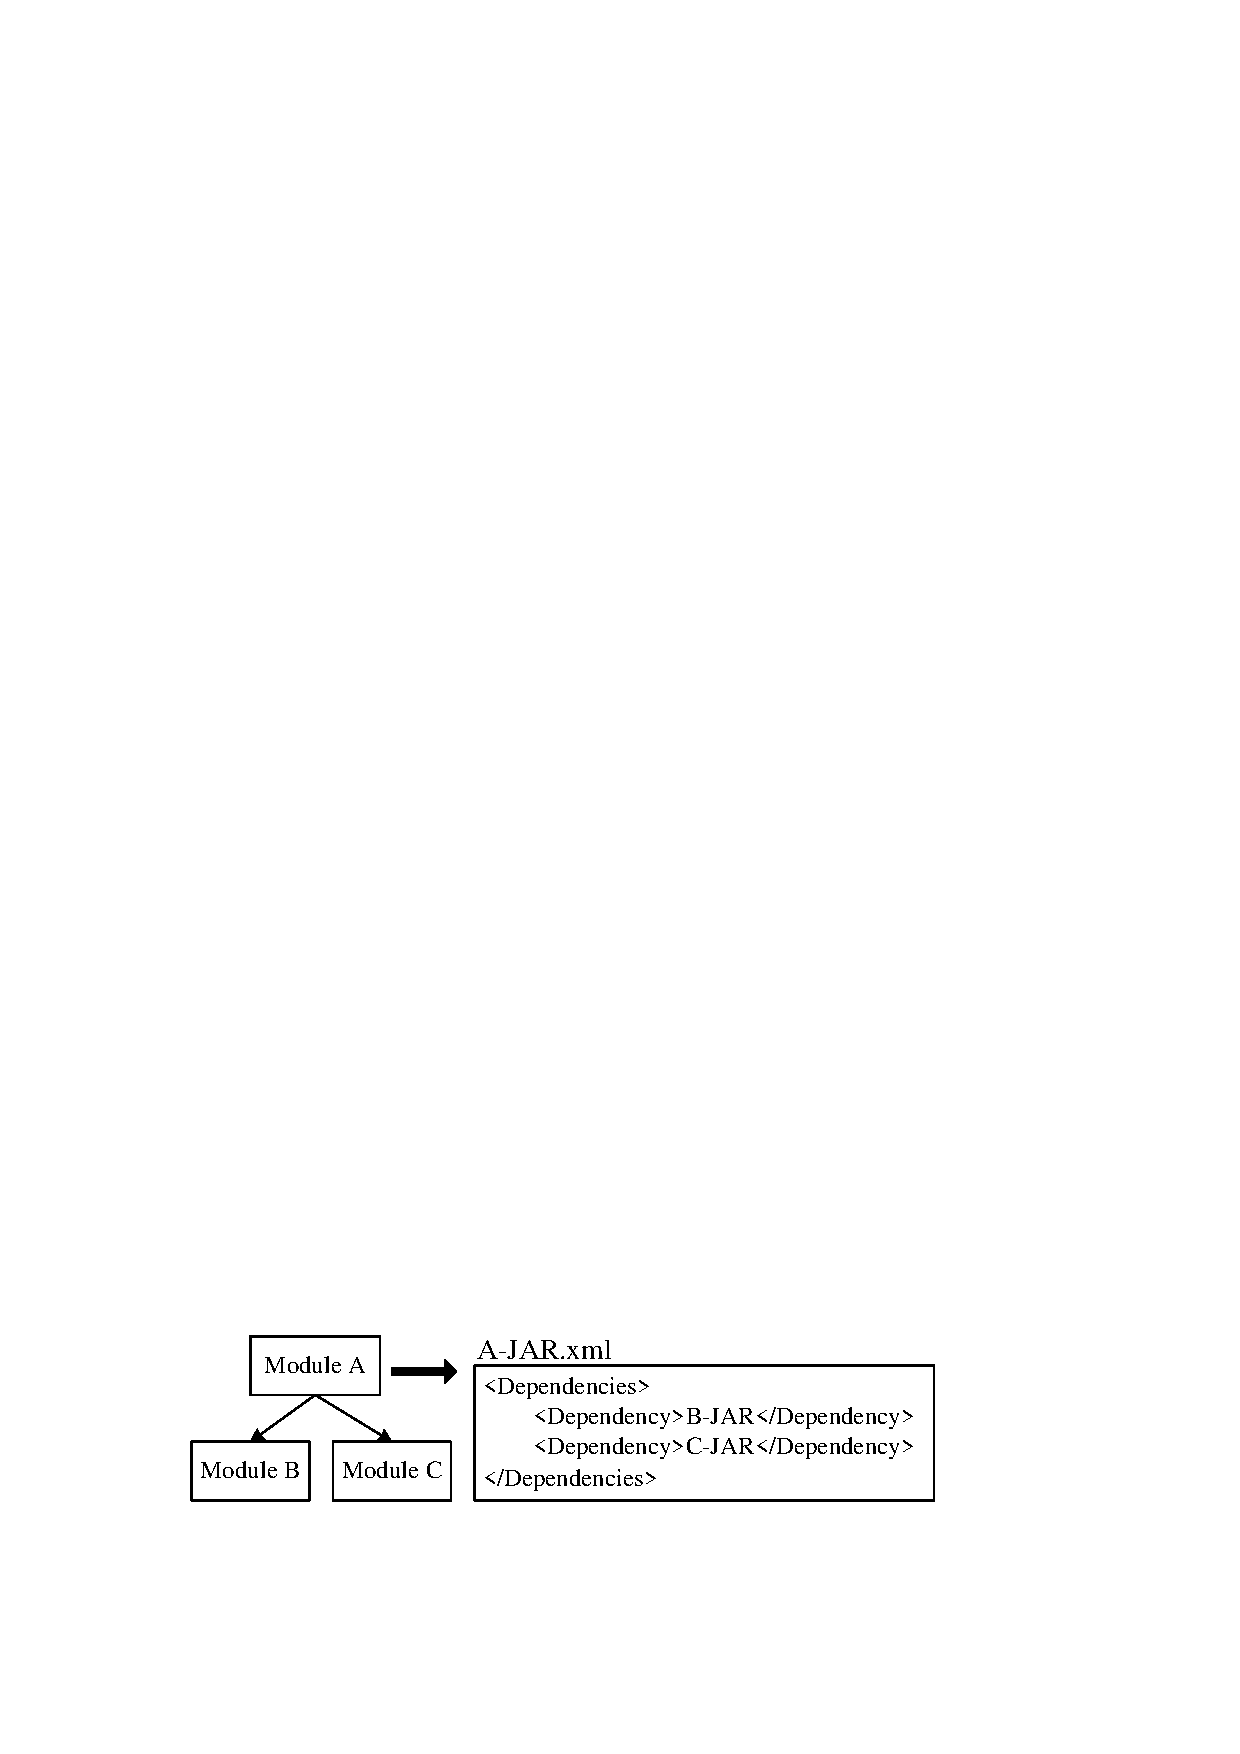
\includegraphics[width=2.2in]{ExampleThree.pdf}
\caption{a modular application with three modules}
\label{fig:example_abc}
\end{figure}


However, providing such a explicit model for dependencies is tedious, especially for the large-scale enterprise modular applications. Actually some component technologies have mechanisms to specify the inter-relationship between components. For example, EJB provides resource injection mechanism\cite{DI} as component assembling. If the module has a description for this kind of dependency, it can be used to find out the dependency between two modules. Then the dependency is recorded in the dependency mapping table, which provides dependency reconstruction with dependency information in the hot deployment. But the injections cannot reflect all the dependencies. For example, some modules can be SPI (service provider interfaces) and other modules are the implementation for those interfaces. In this case, they are still dependent but no component level injections are used to describe this. That means the dependency mapping table cannot record all the dependencies we want, so that dependency reconstruction propably cannot solve the calling failure problems that we discussed before.

For this case, application servers can obtain the module dependencies by the deploying order. The correct deploying order should make each module meet dependencies before deployment. The order of the modular application in Fig. \ref{fig:example_abc} may be B-C-A or C-B-A, because the dependent module A must be deployed after the depended modules B and C. From the deploying order, we cannot record all the dependencies preciously, but we can redeploy all the possible dependent modules for dependency reconstruction. If the order is C-B-A and module C is hot deployed, redeploying module B and module A is a reliable way to reconstruct dependencies, even though there is no need to update module B.

In summary, although reconstruction in application servers can solve the problems of calling failure, there are some disadvantages in this approach.
Not all the dependencies can be obtained during deployment process and be recorded in the dependency mapping table without static profiles.
Dependencies of inheritance or general reference cannot be detected by servers.
So application servers cannot reconstruct these kinds of dependencies and the broken dependencies still exists in most of modular applications.
In addition, this dependency reconstruction is a coarse granularity way to reconstruct and hot deploy modules.
Unlike the depended modules, the dependent modules don't need updating and being redeployed is just for reconstructing dependencies.
So all the dependent modules will be handled through plenty of steps from the deployment process.
This causes application servers inefficient and also causes hot deployment inflexibility.


%// give the overview of the JBoss AS extension.
%// the deployment process, how to obtain dependencies
%// disadvantages
 
 
\section{Dependency Reconstruction with Class Loaders\label{sec:reconstructionCL}}

As we can see, building the dependency reconstruction process into the deployment process suffers from inefficiency or even infeasibility. 
Because each module has its own class loader, the dependencies of modules are just the dependencies of class loaders. 
It is more direct to have the class loaders to maintain the dependencies among the modules that they are responsible to load. 


\subsection{Class Loading Respecting Dependency}

Designing a class loading mechanism for modular applications involves three basic considerations. Firstly, the loader should be able to load the classes in the modules correctly. Secondly, the loader should able to resolve the dependencies among classes from different modules. Lastly, the loaders should be able to reconstruct the dependencies upon some of the modules are update later. 
The loading process for one module can be defined as three steps:
\begin{itemize}
\item Try use the system loaders to load
\item Try use its dependent class loaders to load
\item Try use itself to load
\end{itemize}

The first step is in charge of the loading of fundamental classes, such as those in java.*, with system class loaders respecting the parent delegation policy\cite{parent_delegation}. By this means, the safety and uniqueness of system classes will be guaranteed. This loading strategy gives priority to load classes by parent class loader. \emph{Bootstrap ClassLoader} has the highest priority and the next is \emph{Extension ClassLoader} and \emph{System ClassLoader}. 

If the loading class is not a fundamental class, the class loader will try to load it by itself. The classes in the same module are visible to each other. But the class in the same module may have references to the classes that come from different modules, the class loader should delegate the dependent class loaders to resolve the classes for it. We regard the system class loader as a dependent class loader of each module class loader, so that class loaders should use dependent class loaders to load classes before using itself.


\begin{algorithm}[ht]
\caption{function loadClass of module class loader}
\label{alg:module_class_loader}
\begin{algorithmic}[1]
\REQUIRE ~~\\
Fully qualified name of the class: $name$ \\
Request time of class loading: $firstTime$

\ENSURE ~~\\
The loaded class instance: $c$

\STATE $c\leftarrow$\emph{findLoadedClass}($name$)

\IF {$c = null\ \&\&\ visitTime < firstTime$}

	\STATE $visitTime\leftarrow currentTime$
	
	\FOR {\textbf{each} class loader $dep$ in $depList$}
		
		\STATE $c\leftarrow dep.$\emph{loadClass}($name$, $firstTime$)
		
		\IF {$c\ne null$}
			
			\STATE \textbf{return} $c$

		\ENDIF
	
	\ENDFOR

	\STATE $c\leftarrow$\emph{findClass}($name$)

\ELSE
	
	\STATE \textbf{return} $c$

\ENDIF


\end{algorithmic}
\end{algorithm}


Algorithm \ref{alg:module_class_loader} shows the module class loader how to load classes in modular applications.
Here is the definition of module dependency.
In modular applications, a module can be defined as $M=<C, L, R>$. 
$C=\{c_1, c_2, c_3\cdots\}$ is the set of classes in that module. 
$L$ is a module class loader to load all the classes in the class set $C$.
$R=\{M_1, M_2, M_3\cdots\}$ is the set of its dependencies against other modules. 
Take the division modular application shown in Fig. \ref{fig:example} as an example, Compute.jar is a dependent module and $R = \{Validator.jar\}$, because class \emph{ComputeBean} calls the method \emph{iszero} in class \emph{ValidatorBean} and these two classes are in different modules.
Validator.jar is a depended module used to verify the divisor and $R = \emptyset$, which means Validator.jar doesn't depends on any modules.

Under the definition of module dependency, class set $C$, class loader $L$ and dependencies $R$ of each module $M$ are determined from the dependency graph, which can be created by the static module profiles before class loading.
Moreover, we can obtain the dependent class loader list of $L$ from each class loader of each module in $R$, which represents \emph{depList} in Algorithm \ref{alg:module_class_loader}. 
We should note that the module class loaders may delegate each other due to the \emph{depList} with circles, which will cause endless loop.
So we take a simple solution to detect circles in the algorithm of loading classes.
In Algorithm \ref{alg:module_class_loader}, $firstTime$ is a timestamp which records the time for the beginning of the class loading and $visistTime$ is a timestamp which is used to represent the last visit time for using this class loader. 
If the condition $visitTime < firstTime$ is not \emph{true}, there is no need to delegate dependent class loaders to load because they have already been delegated.
In this way, the class loaders will not delegate each other, even if there exists interdependence among modules.

When updating is detected, some affected class loaders and dependencies must be modified.
However, modifying the changing class loaders and their dependencies is not enough because dependencies may be broken while hot deploying depended modules.
For instance, if Validator.jar is updated, in order to reconstruct dependencies, all of modules which depend on Validator.jar also require to be updated even though they have no new versions and users don't want to update them.
So we reconstruct the dependencies for Validator.jar by updating these class loader of affected modules.
But reconstruction is not finished because other modules may depend on these updated modules.
We need to reconstruct their dependencies too in the same way, until there is no original modules which depend on any of the updated modules.
All the affected modules should own their new class loader instance instead of the old one, because the old class loader has the cache of old classes and it cannot load the new classes with the same name.
Replacing the old class loaders is the most convenient way to update modules and reconstruct dependencies.
Meanwhile, updating the old class loader instances and dependencies is necessary.



\subsection{Constructing the Dependency Graph}

The dependency graph can be created by the module profiles like the profiles for reconstruction in servers.
It is a static way to manage and reconstruct the dependencies.
But editing module profiles is a quite messy work when modular applications are composed of hundreds of modules.
Dynamic dependency management avoids this work because it has a loading queue to make a try when loading classes.
The loaded class will be placed in the repository and the unloaded class will enter the loading queue again to wait for the next loading.
Due to continuous trying, we can obtain dependencies of all the classes (modules) and construct the dependency graph by an adaptive way.
The loading rules extend the basic loading process and the priority order is described in the following: 
\begin{itemize}[\IEEEsetlabelwidth{9}]
\item[1)] Try to use the system class loader to load it, if the class name begins with java.*.
\item[2)] Try to use its own class loader to load it.
\item[3)] Try to use its dependent class loaders to load it.
\item[4)] Try to use the class loaders which have already loaded other classes in the repository. 
\end{itemize}

\begin{figure*}[ht]
\centering
\subfloat[loading ComputeBean]
{
	\label{fig:subfig:a}
	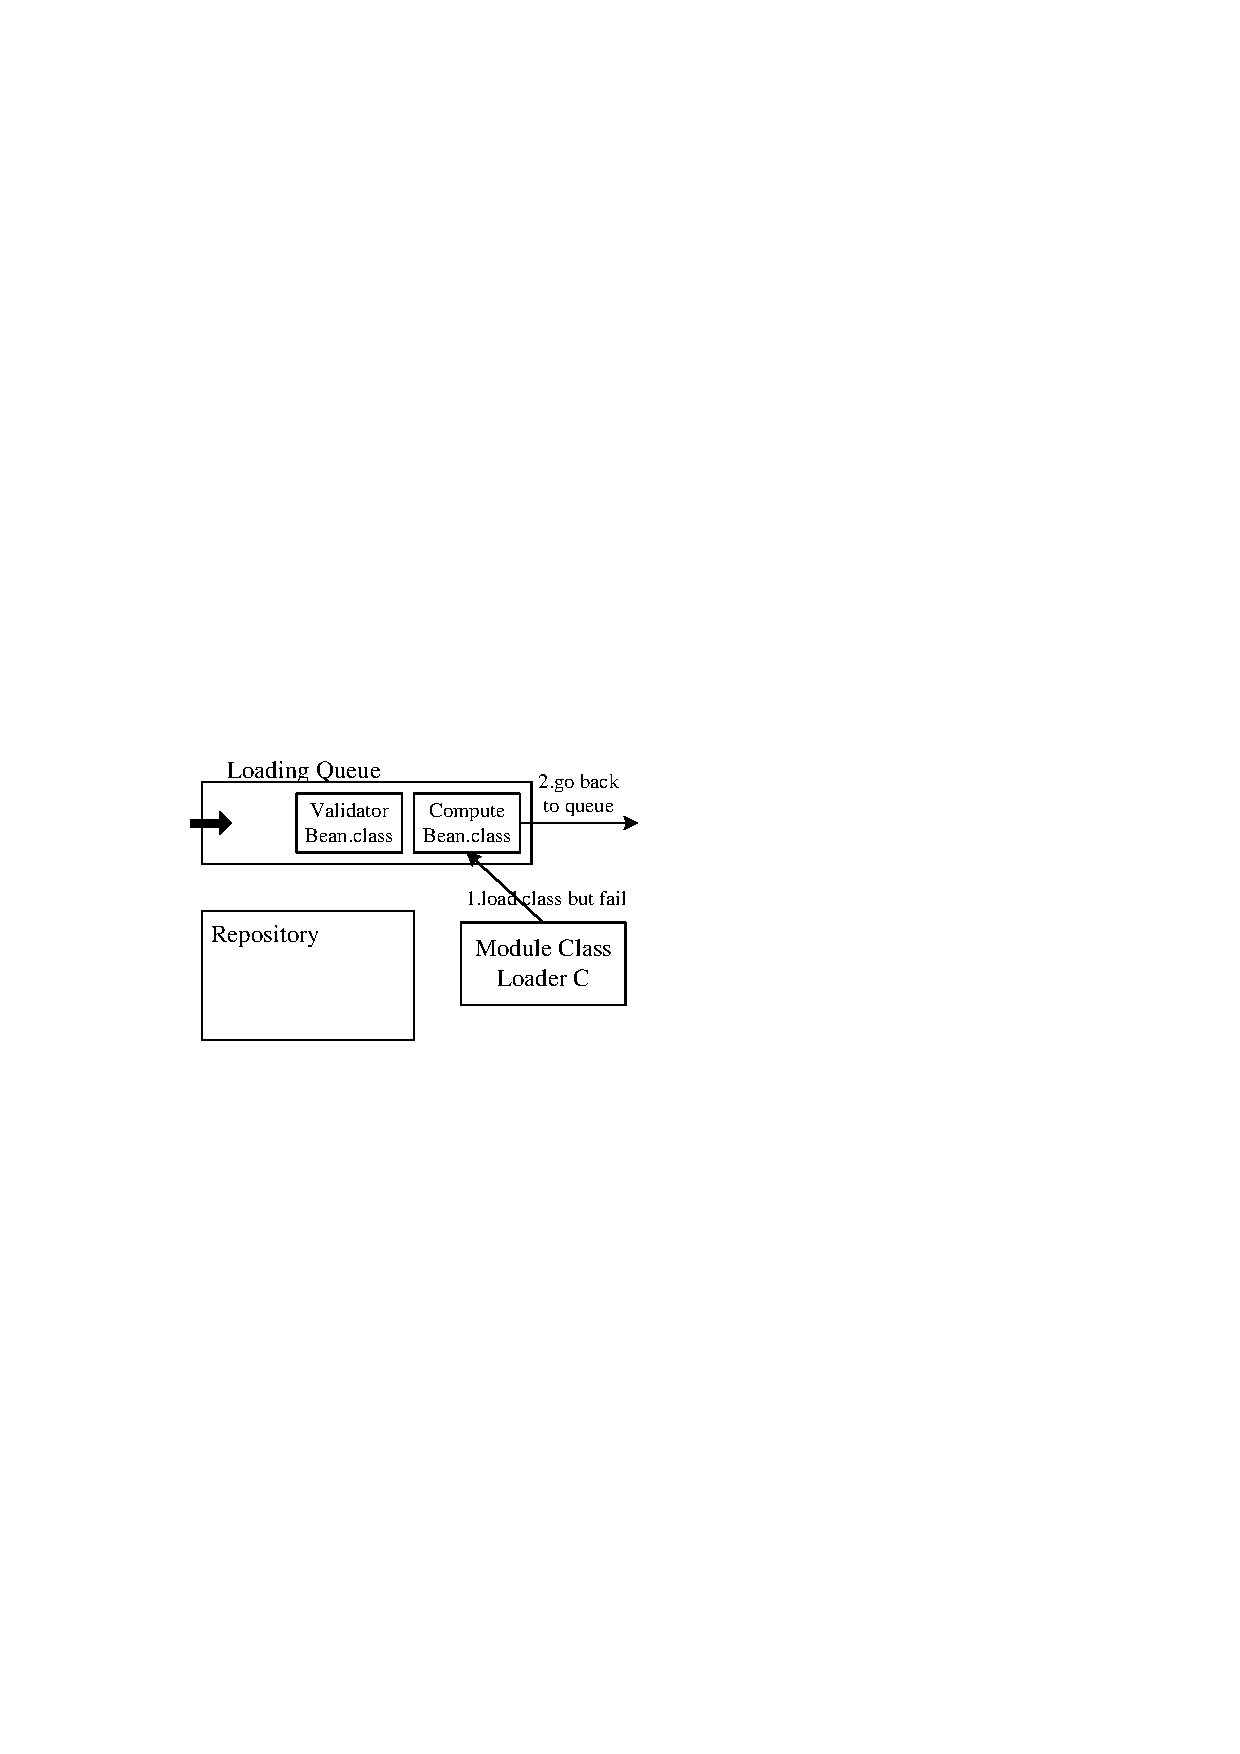
\includegraphics[height=1.4in]{LoadingQueueA.pdf}
}
\hfil
\subfloat[loading ValidatorBean]
{
	\label{fig:subfig:b}
	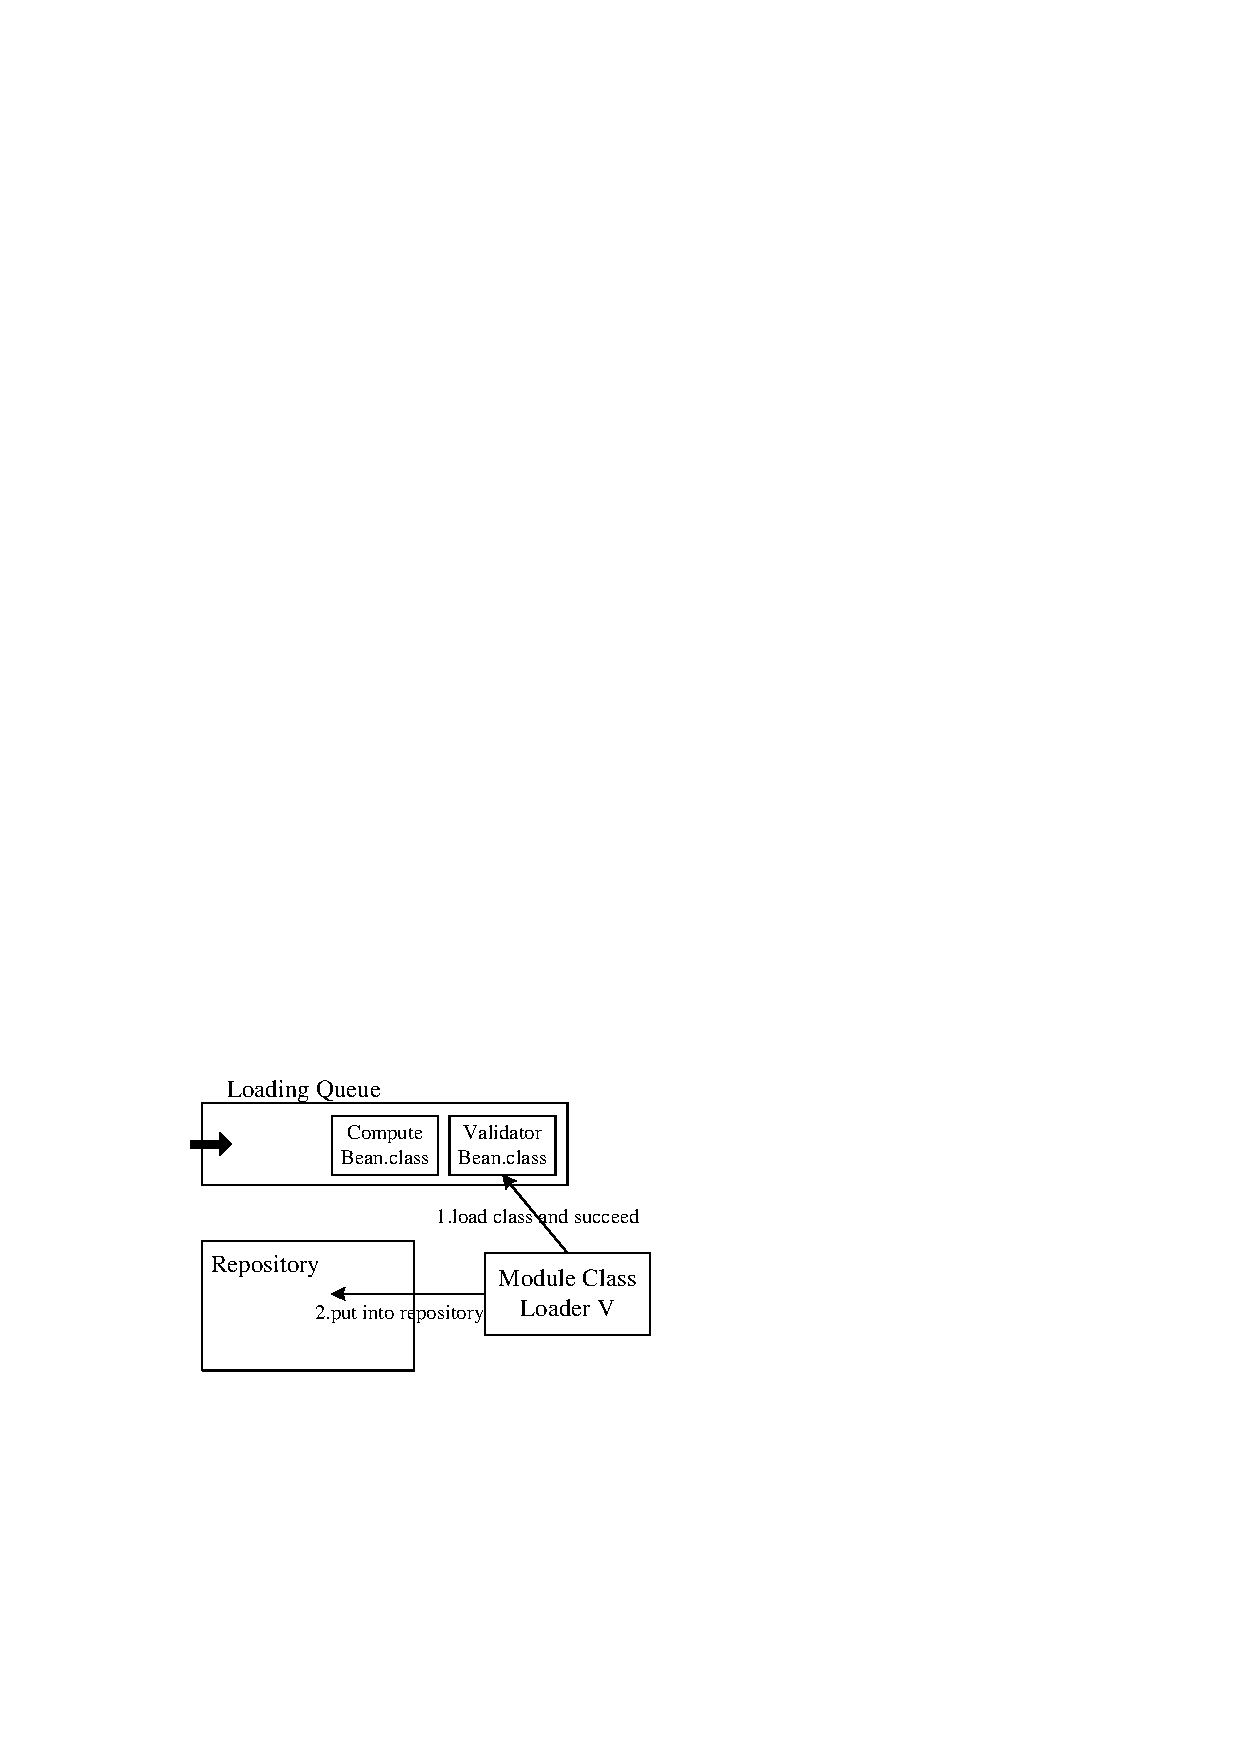
\includegraphics[height=1.4in]{LoadingQueueB.pdf}
}
\hfil
\subfloat[loading ComputeBean again]
{
	\label{fig:subfig:c}
	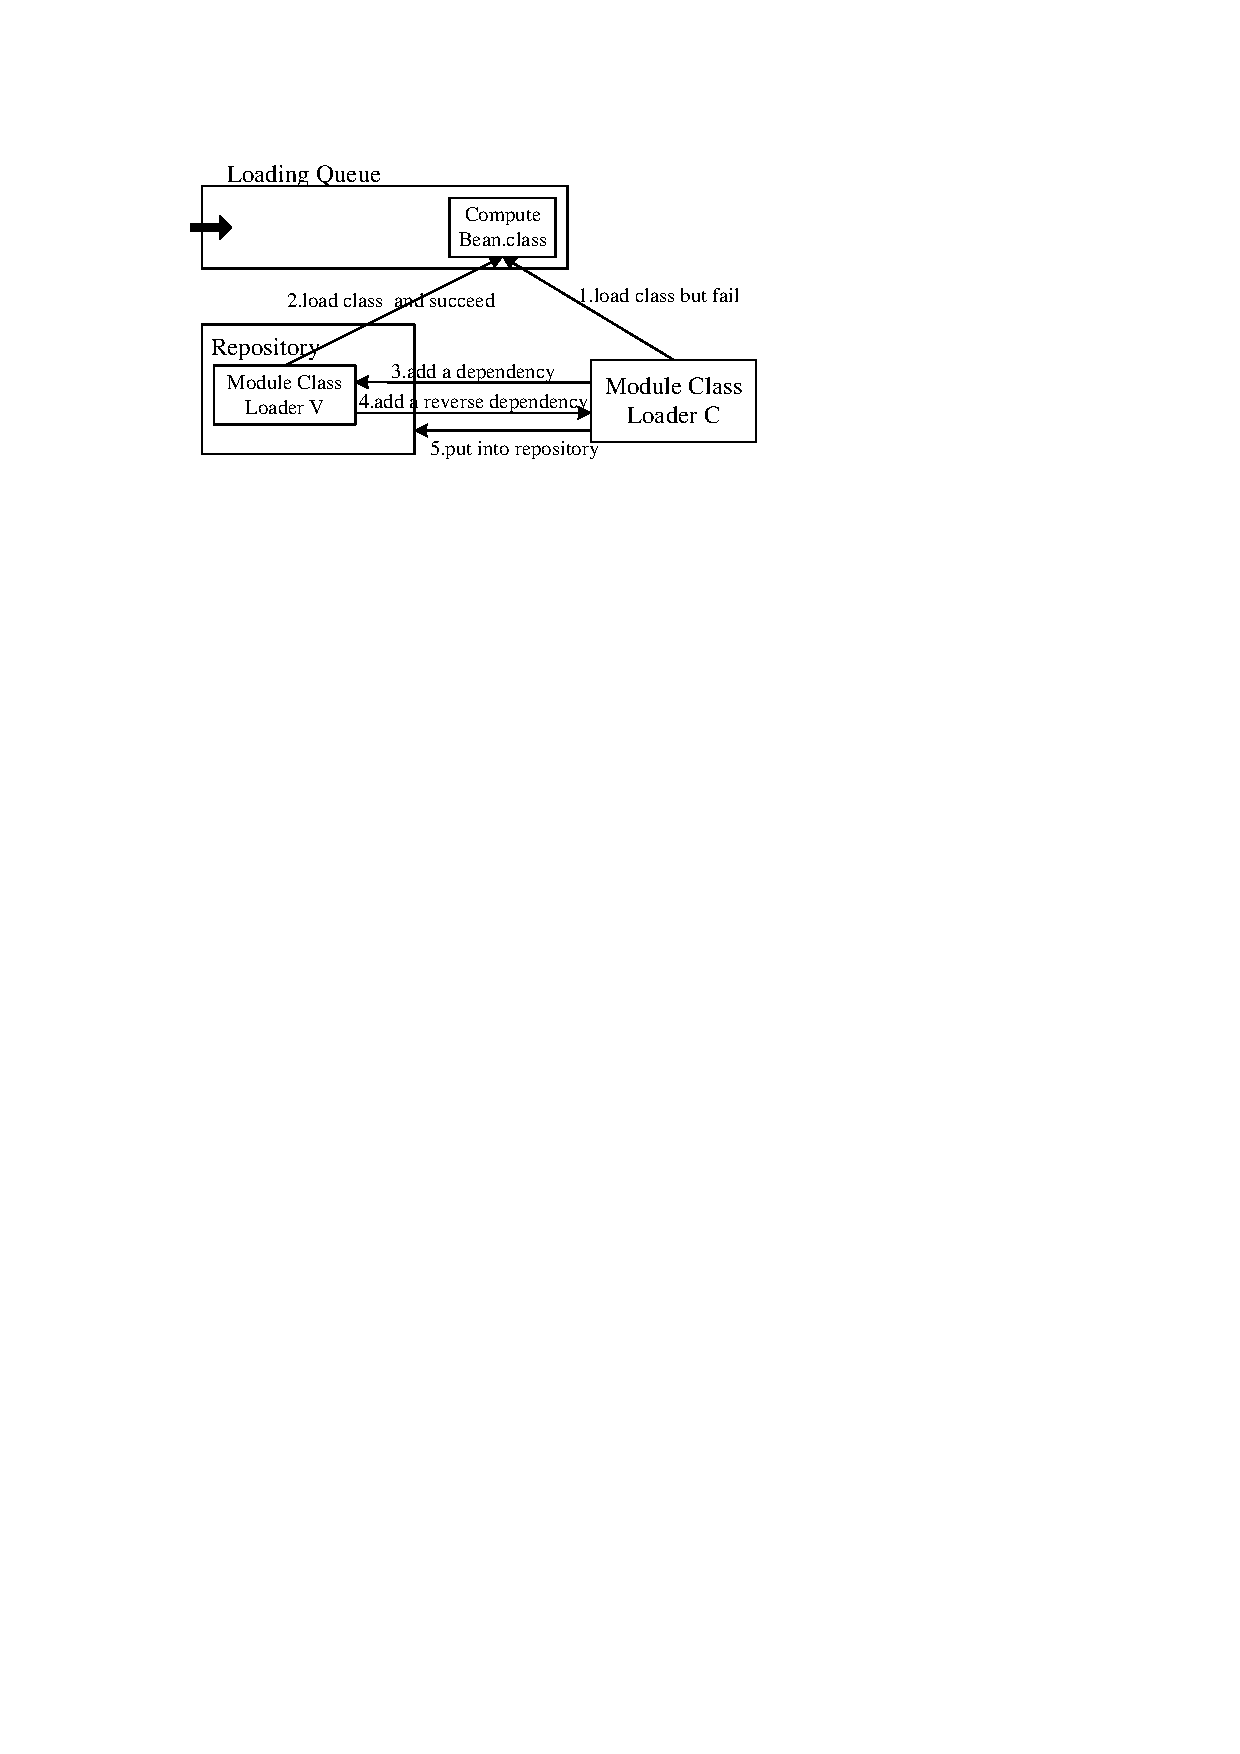
\includegraphics[height=1.4in]{LoadingQueueC.pdf}
}
\caption{details of loading class and constructing dependency}
\label{fig:loading_queue}
\end{figure*}

Fig. \ref{fig:loading_queue} shows the loading classes process of the division application that we used before. 
There are two classes \emph{ComputeBean} and \emph{ValidatorBean} in the application. 
We put them into the loading queue and try to load \emph{ComputeBean} at first. 
Due to the dependencies, module class loader $C$ which belongs to Compute.jar fails to load it. 
Class \emph{ComputeBean} should go back to the loading queue again to wait the next loading, which is described as Fig. \ref{fig:subfig:a}. 
Then it is turn to load Class \emph{ValidatorBean} in Fig. \ref{fig:subfig:b}. 
Module class loader $V$ loads it successfully, so we add the class loader into the repository. 
With more classes loaded successfully, more class loaders will be put in the repository and they help to load other classes. 
Thus, \emph{ComputeBean} can be loaded successfully at the second time by the class loader in the repository as presented in Fig. \ref{fig:subfig:c}.
If a class loader in the repository loads the other class successfully, that means it is the dependent class loader of the other class loader and the dependency is created in the class loader incidentally. 
Finally, the loading queue becomes empty and all the classes are loaded with the dependencies.
Without static profiles, module class loaders create dependencies dynamically while loading classes.

If hot deployment happens, the old version classes in the repository must be removed and their related dependencies must be dropped. 
Then, the new version classes are also placed in the loading queue to wait for loading. 
Dependency reconstruction in dynamic dependency management also needs to find out all the dependent modules group by group. 
No matter whether these modules have the new version, they must be removed in the repository and put their classes in the loading queue to be reloaded. 
So, all the broken dependencies will be reconstructed by taking the place of the original class loaders and their dependent class loaders. 

\begin{figure}[ht]
\centering
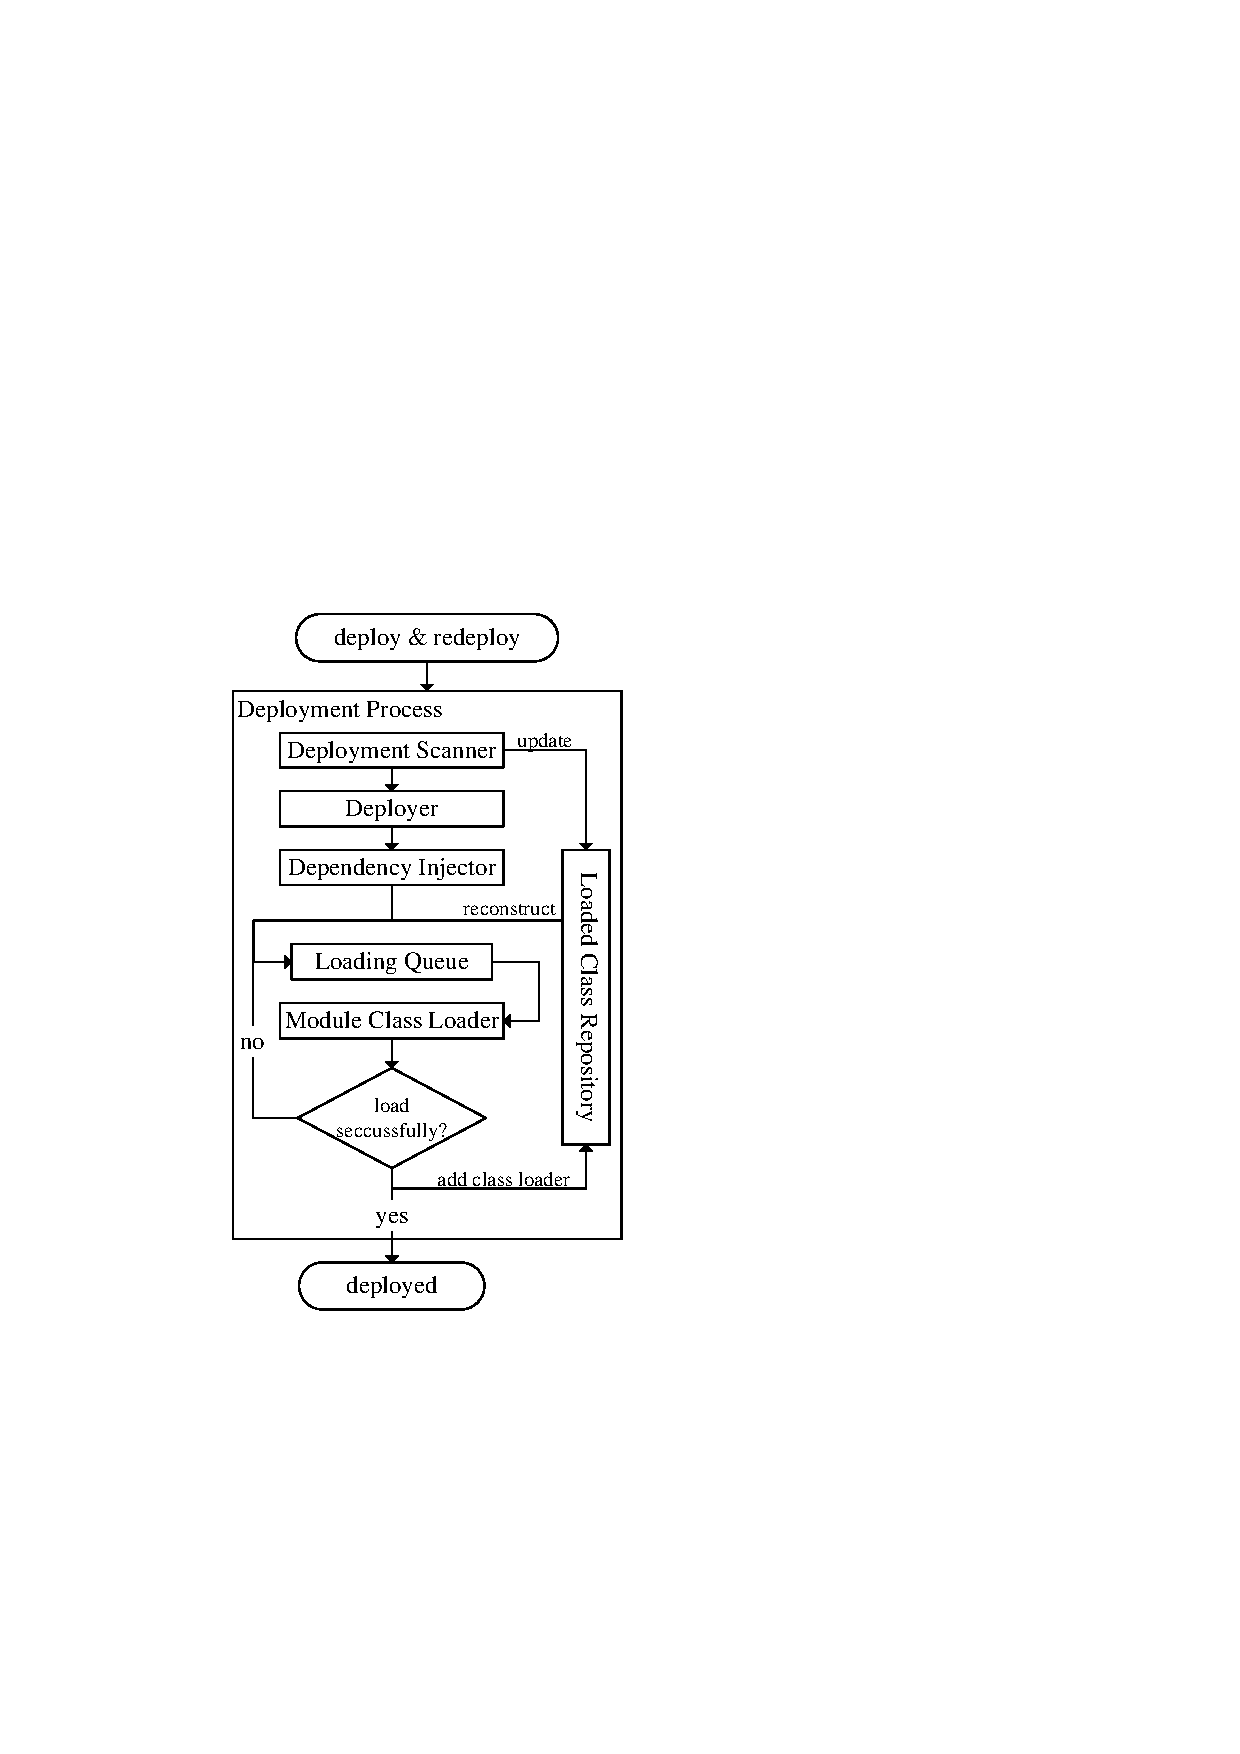
\includegraphics[width=2.0in]{ProcessReconstructionCL.pdf}
\caption{dependency reconstruction with class loaders}
\label{fig:reconstruction_CL}
\end{figure}

Fig.\ref{fig:reconstruction_CL} shows the whole process of hot deployment with dependency reconstruction with class loaders. 
The affected modules only update their module class loaders and the affected classes need to be reloaded through the loading queue, so that we save the partial cost of redeployment process for the dependent modules which are still the old versions. 
Even though adaptive way to load class is time consuming, avoiding editing dependencies in the module profiles is a time saving thing for developers of modular applications or administrators of application servers.


\subsection{Lazy Reconstruction}

Lazy reconstruction makes module class loaders more flexible.
Comparing with immediate reconstruction, the class loader with lazy reconstruction delays dependency reconstruction when hot deployment happens.
This class loader doesn't reconstruct dependencies at once. 
So all the affected class loaders only mark as invalid class loaders and none of class loaders are updated after hot deployment.
Dependency reconstruction will happen when applications are executed.
Because in this time, the class loader with lazy reconstruction has to reconstruct dependencies to ensure the correctness of applications.
If the class loader is invalid, we should update and reconstruct it before using it to load classes. 
The algorithm of loading class is described in Algorithm \ref{alg:lazy_reconstruction}, which uses the loading rules we discussed before.
The dependency reconstruction process is also as the same as the reconstruction process of the class loader with immediate reconstruction.
Their main difference is their reconstruction time.
With lazy reconstruction, the class loader will reconstruct dependencies when applications are executed, so that it may save the time of hot deployment and avoid reconstruction if users never execute some modules after updating them.

\begin{algorithm}[ht]
\caption{function loadClass with lazy reconstruction}
\label{alg:lazy_reconstruction}
\begin{algorithmic}[1]
\REQUIRE ~~\\
Fully qualified name of the class: $name$ \\

\ENSURE ~~\\
The loaded class instance: $c$

\STATE $c\leftarrow$\emph{findLoadedClass}($name$)

\IF {$c = null$}
	
	\IF {$name.$\emph{startWith}("java.")}
	
		\STATE $c\leftarrow SystemClassLoader.$\emph{loadClass}($name$)
	
		\IF {$c \ne null$}

			\STATE \textbf{return} $c$
	
		\ENDIF

	\ELSE

		\STATE $c\leftarrow$\emph{findClass}($name$)

		\IF {$c = null$}

			\FOR {\textbf{each} class loader $dep$ in $depList$}

				\STATE $c\leftarrow dep.$\emph{loadClass}($name$)

				\IF {$c\ne null$}
			
					\STATE \textbf{return} $c$

				\ENDIF
			
			\ENDFOR

			\FOR {\textbf{each} class loader $cl$ in $repository$}
				

				\IF {$cl.$\emph{valid} = false}

					\STATE $cl\leftarrow$\emph{reconstruct}($cl$)
				
					\STATE $cl.$\emph{valid}$\leftarrow$true

				\ENDIF

				\STATE $c\leftarrow cl.$\emph{loadClass}($name$)

				\IF {$c\ne null$}

					\STATE $depList$.\emph{add}($cl$)
			
					\STATE \textbf{return} $c$

				\ENDIF
			
			\ENDFOR
	
	
		\ELSE

			\STATE \textbf{return} $c$

		\ENDIF

	\ENDIF

\ELSE

	\STATE \textbf{return} $c$

\ENDIF


\end{algorithmic}
\end{algorithm}


%// how to reconstruct, (we can find the dependencies in the class loader)
%// why updating class loaders is neccessary
%// our contribution


\section{Evaluation\label{sec:evaluation}}
In this section, we do some evaluations on efficiency, dynamic feature and flexibility for our technology of hot deployment with dependency reconstruction.

\subsection{Experiment}
Mainstream application servers only support hot deployment of standalone applications, which cannot satisfy the requirement of modular applications.
Hot deployment with dependency reconstruction can ensure the correctness of the modular applications.
We use a simple division modular application in Fig. \ref{fig:example} to evaluate the hot deployment with dependency reconstruction.
And our experimental environment is following:
\begin{itemize}[\IEEEsetlabelwidth{9}]
\item[1)] OS: Ubuntu 12.04
\item[2)] JDK: Java Version "1.6.0\_24"
\item[3)] IDE: Eclipse IDE for Java EE Developers
\item[4)] AS: JBoss AS 5.1.0 \& JBoss AS 5.1.0 extension (Reconstruction in AS)
\end{itemize}

We start the application server and deploy two session beans called Compute.jar and Validator.jar and we can compute division correctly through this modular application.
Then we only update Validator.jar.
After hot deployment, the application in JBoss AS 5.1.0 will throw the EJB exception when we use Compute.jar to do division of two numbers.
However, JBoss AS 5.1.0 extension reconstructs broken dependencies and redeploys Compute.jar, so that we can make the calculation without exception.
Dependency reconstruction guarantees the correctness of hot deploying dependent modules in modular applications.

Comparing with JBoss AS 5.1.0, the application server extension, using dependency reconstruction in application servers, needs more time to hot deploy modules because the server searches dependencies in the dependency mapping table and deploys more dependent modules.
But this type of dependency reconstruction can guarantee the correctness of hot deployment without restarting application servers.
Obviously, the hot deployment with dependency reconstruction which can avoid restarting servers is more efficient.


\subsection{Efficiency}


\begin{table*}
\centering
\caption{time cost of deployment stages}
\label{tab:stage}
\begin{tabular}{|c|c|c|c|c|}
\hline
\emph{Module Name}	&	\emph{Configuration Stage}	&	\emph{Distribution Stage}	&	\emph{Total Time}	&	\emph{Promotion Rate}\\
\hline
\hline
Compute.jar		&	13ms			&	33ms			&	46ms			&	28.3\%\\
\hline
Validator.jar		&	12ms			&	29ms			&	41ms			&	29.3\%\\
\hline
pestore.jar(1.1.2)	&	34ms			&	236ms			&	270ms			&	12.6\%\\
\hline
pestore.jar(1.3.2)	&	24ms			&	113ms			&	137ms			&	17.5\%\\
\hline
netboot.war		&	19ms		 	&	65ms			&	84ms			&	22.6\%\\
\hline
persistent-service.sar 	& 	14ms 			&	35ms			&	49ms			&	28.6\%\\
\hline
ejb-management.jar	& 	12ms		 	&	283ms			&	295ms			&	4.1\%\\
\hline
derby-plugin.jar	&	16ms			&	16ms			&	32ms			&	50.0\%\\
\hline
threaddump.war		&	10ms			&	52ms			&	62ms			&	16.1\%\\
\hline
jbossts-tools.sar	&	21ms			&	87ms			&	108ms			&	19.4\%\\
\hline
jbossxts.sar		&	52ms			&	860ms			&	912ms			&	5.7\%\\
\hline
\end{tabular}
\end{table*}


Reconstruction in application servers is a native way to solve calling failures because many dependent modules with original versions are redeployed after the depended modules.
However, most of the work in redeploying dependent modules makes no sense except class loading in the modules.
Reconstruction with class loaders improves updating efficiency because dependency management is handled in the class loader, which means a lot of work in the redeployment process can be eliminated when reconstruction happens.

According to deployment specification\cite{jsr88}, deployment is typically a three-stage process: configuration, distribution and start execution.
We focus on the first two stages in our experiments.
Deployment context of modules are created in configuration stage, but they are not changed when redeployment of dependent modules happens.
We use the original context and only update its module class loader before distribution stage which is responsible for installing modules and loading classes.
So we save the time used to create and set the deployment context in the redeployment process.

Table \ref{tab:stage} shows the cost of redeployment in these two stages for some modules and applications.
Compute.jar and Validator.jar are two session beans which constitute a modular application for dividing calculation in Fig. \ref{fig:example}.
Java Pet Store\cite{java_pet_store} is a sample well-known application from the J2EE\cite{j2ee}, so it is also one of our subjects.
The rest testing modules are services of JBoss, which can be found in the directory of JBossAS 5.1.0 Release named \emph{examples}.
We hot deploy them when the application server is running and calculate the time cost of the configuration stage and distribution stage.
In our approach of reconstruction with class loaders, the time cost of the configuration stage will be saved when hot deployment happens.
The efficiency is highly improved according to the promotion rate of Table \ref{tab:stage}.
Moreover, dependent modules won't update themselves in the deployment directory and the scanning time, which is 5 seconds as default configuration, is saved and that means applications don't require to wait for the class loading delay of dependent modules. 


\begin{table*}
\centering
\caption{performance of flexible reconstruction}
\label{tab:flexibility}
\begin{tabular}{|c|c|c|c|c|}
\hline
\emph{Reconstruction Strategy}	& \emph{Deploy and Execute All}	& \emph{Redeploy and Execute All} & \emph{Redeploy and Execute One}\\
\hline
\hline
immediate reconstruction 	&	94ms				&	141ms				&	52ms\\
\hline
lazy reconstruction 	&	92ms				&	138ms				&	43ms\\
\hline
\end{tabular}
\end{table*}


\subsection{Dynamic Feature}
Comparing with the class loader based on static dependency management, the class loader can also obtain the dependencies of modules in the dynamic way.
By several attempts, we can create the dependency graph on the basis of whether the class is loaded successfully.
Developers don't need to provide the module profiles to describe the dependencies of the modules.
The dependencies are managed and reconstructed dynamically at any time.

Actually, static dependency management is more efficient than dynamic dependency management in terms of deployment and redeployment time.
Distribution stage accounts for a large proportion of the total deployment process according to Table \ref{tab:stage}.
In dynamic way, the class loader may try to load a class for many times if this class depends on other classes which are packaged in different modules.

However, the advantage of dynamic feature is reducing management of modules for developers.
As we know, enterprise applications probably contain hundreds of modules and complex dependencies.
It is annoying for developers to create and manage profiles of each module if there are no reliable automatic tools for generating them.
Additionally, dynamic feature makes hot deployment more flexible, which we will talk about in the following part.


\subsection{Flexibility}

The class loader is an important part in application servers based on J2EE.
Reconstruction with class loaders make hot deployment more flexible.
On the one hand, dynamic dependency management allows class loaders to construct dependencies in the attempt to load classes without profiles.
On the other hand, reconstruction can be carried out at any time before execution of applications.
With immediate reconstruction, the class loader will reconstruct dependencies in the process of hot deployment, which means the class loader will finish reconstructing dependencies when the application server completes hot deployment.
In contrast, the class loader with lazy reconstruction, which should be reconstructed, is only marked as invalid when hot deployment happens.
The class loaders and their dependencies won't be updated until the applications start to be executed.
So, we handle invalid class loaders and reconstruct them at the time of application execution.
Comparing with immediate reconstruction, lazy approach delays reconstruction and increase the flexibility of reconstruction.

In a particular application scenario, the class loader with lazy reconstruction has a good performance. 
We compare dependency reconstruction between immediate and lazy approach through experiments.
We choose a simple modular application with three modules A, B and C, shown as Fig. \ref{fig:example_abc}.
Then we copy this application for 20 times and build 20 modular applications with identification from 1 to 20.
In the experiment, we deploy 20 applications with 60 modules in the server and then we hot deploy module B of all the applications.
To ensure the correctness of applications, module A and B need to be reconstructed.
With lazy reconstruction, we execute all the applications after redeployment so that all of class loaders finish reconstructing.
If we execute one application, only the class loaders of this application modules will complete reconstruction.
So, the time of hot deployment and execution decreases in Table \ref{tab:flexibility}. 



\section{Related work\label{sec:relatedwork}}

The concept of modularity was proposed a long time ago by Divid Parnas\cite{Divid_specification}.
He gave two main criteria\cite{Divid_criteria} to be used in decomposing systems into modules in 1972.
They were making each major step in the processing module and using information hiding as a criterion.
After that, people gradually changed the way of developing software.
And Modularity impacts on development, deployment, operation, maintenance in software engineering until now.
So, many researchers focus on modularity and modular applications in all fields of software engineering, such as software metric\cite{module_metric} and software testing\cite{module_test}.
Even some new technologies and concepts (e.g. AOP\cite{module_aop} and cloud\cite{module_cloud}) of software engineering also have related to modularity and modular applications.

Although many researchers dedicated to the study of hot deployment, most of the work focused on the hot deployment of distributed heterogeneous environments\cite{related_hot_1, related_hot_2, related_hot_3, related_hot_4}.
They solved problems about the dynamic service creation, service life cycle management and other issues based on OGSA (Open Grid Service Architecture).
In terms of dependency injection, most of the work focused on the dependency injection mechanism and its performance in different environments\cite{related_DI_1, related_DI_2, related_DI_3}.
They involved a number of fields, such as distributed applications, design patterns, and software maintenance.
In contrast, our work proposes a technology of hot deployment with dependency reconstruction, which makes hot deployment more flexible and efficient.

Improving abilities of application servers through component extension is not a new idea.
For example, Li et al. advocated an on demand approach of deploying services in application servers\cite{related_AS_1} and they even proposed an approach to make an application server well-structured and dynamic\cite{related_AS_2}.
And some research focused on refactoring application servers according to application requirements\cite{related_AS_3}.
	
On the other hand, application servers can preprocess modules before modular applications are deployed, which brings many benefits in performance. 
For instance, several modules merge into one module to reduce dependencies\cite{related_merge} or a module splits into several ones in order to reduce the cost of update\cite{related_split}.
It is also helpful to our future work on dependency reconstruction with class loaders.
In this way, we will decrease the granularity of update and reconstruction.


\section{Conclusion and future work\label{sec:conclusion}}
Hot deployment mechanism is one of the typical features of mainstream application servers.
However, they cannot meet the demand with hot deployment of modular applications.
This paper proposes a technology of hot deployment with dependency reconstruction which can solve the problem of hot deploying modular applications in practical engineering projects.
To make hot deployment becomes more flexible and efficient, dependency reconstruction with class loaders is implemented by several ways, including static profiles way, dynamic adaptive loading way and lazy reconstruction way.
Dependencies can be managed and reconstructed when hot deployment happens.
Experiments show that the problems of calling failure can be solved through this technology and the efficiency of application servers is improved.

In future, we will focus on reconstruction with class loaders.
Managing dependencies in class loaders make it possible to decrease the granularity of update and reconstruction.
We can split a module into several sub modules or assemble some modules according their original dependencies.
So reconstruction with class loaders will reduce the granularity of the update and narrow the scope of the hot deployment.
With the more flexible hot deployment, the efficiency of application servers will be highly increased.
Moreover, we will implement dependency reconstruction in the code level\cite{future_Gu}, so that code-level dynamic update will be achieved and it will continue to decrease the granularity of update.

% conference papers do not normally have an appendix
% use section* for acknowledgement
\section*{Acknowledgment}
This work is partially supported by National Basic Research 973 Program(Grant No. 2015CB352202), and National Natural Science Foundation(Grant Nos. 61472177, 91318301, 61321491, 61361120097) of China.

% may modify acknowledgment



% references section
\begin{thebibliography}{9}

\bibitem{app_server}
What is an App Server, \url{http://www.theserverside.com/news/1363671/What-is-an-App-Server}.

\bibitem{jboss}
JBoss Application Server, \url{http://www.jboss.org}.

\bibitem{weblogic}
Oracle WebLogic Server, \url{http://www.oracle.com/technetwork/middleware/weblogic/overview/index.html}.

%\bibitem{middleware_reliability}
%Huang, Gang, et al. "Simulation-based analysis of middleware service impact on system reliability: Experiment on Java application server." Journal of Systems and Software 84.7 (2011): 1160-1170.

\bibitem{standard_cl}
Taylor, B. "Java Class Loading: The Basics." (2003).

\bibitem{module_cl}
Gangadharan, Binod Pankajakshy, Srikanth Padakandla, and Sivakumar Melapannai Thyagarajan. "Hot deployment of shared modules in an application server." U.S. Patent No. 7,721,277. 18 May 2010.

\bibitem{jboss_class_loader}
The JBoss JMX Microkernel, \url{http://docs.jboss.org/jbossas/jboss4guide/r5/html/ch2.chapter.html}.

\bibitem{EJB}
JSR 220: Enterprise JavaBeans\textsuperscript{\texttrademark} 3.0, \url{https://www.jcp.org/en/jsr/detail?id=220}.

\bibitem{jvm}
Java Virtual Machine, \url{http://java-virtual-machine.net/sun-java-virtual-machine.html}.

\bibitem{jvm_book}
Zhiming, Zhou. "Understanding the JVM Advanced Features and Best Practices." (2011).

\bibitem{jvm_specification}
The Java Virtual Machine Specification, \url{http://docs.oracle.com/javase/specs/jvms/se7/html}.

\bibitem{DI}
Fowler, Martin. "Inversion of control containers and the dependency injection pattern." (2004).

%\bibitem{deployment_process}
%Olliges, Sascha. Runtime Reconfiguration in J2EE Systems. Diss. Master Thesis supervised by Jasminka Matevska and Wilhelm Hasselbring, University of Oldenburg, Germany, Department of Computing Science, Software Engineering Group, 2005.

\bibitem{parent_delegation}
Rohit Chaudhri. "Understnding the Java Classloading Mechanism." Java Developer's Journal Vol.8, Issue 8, p.16.

%\bibitem{class_loader_patent}
%Meduri, Subbarao K., Thomas Edward Musta, and James Lee Van Oosten. "Collaborative classloader system and method." U.S. Patent No. 7,870,546. 11 Jan. 2011.

\bibitem{jsr88}
JSR-000088, Deployment API Specification, \url{http://jcp.org/aboutJava/communityprocess/mrel/jsr088/index.html}.

\bibitem{java_pet_store}
Java Pet Store, \url{http://www.oracle.com/technetwork/java/petstore1-3-1-02-139690.html}.

\bibitem{j2ee}
Bodoff, Stephanie, ed. The J2EE tutorial. Addison-Wesley Professional, 2002.



\bibitem{Divid_specification}
Parnas, David Lorge. "A technique for software module specification with examples." Communications of the ACM 15.5 (1972): 330-336.

\bibitem{Divid_criteria}
Parnas, David Lorge. "On the criteria to be used in decomposing systems into modules." Communications of the ACM 15.12 (1972): 1053-1058.

\bibitem{module_metric}
Kazemi, Ali, et al. "A metric suite for measuring service modularity." Computer Science and Software Engineering (CSSE), 2011 CSI International Symposium on. IEEE, 2011.

\bibitem{module_test}
Judge, Lyndon, et al. "A modular testing environment for implementation attacks." BioMedical Computing (BioMedCom), 2012 ASE/IEEE International Conference on. IEEE, 2012.

\bibitem{module_aop}
Przybyłek, Adam. "Where the truth lies: AOP and its impact on software modularity." Fundamental Approaches to Software Engineering. Springer Berlin Heidelberg, 2011. 447-461.

\bibitem{module_cloud}
Wettinger, Johannes, et al. "Enabling Dynamic Deployment of Cloud Applications Using a Modular and Extensible PaaS Environment." Cloud Computing (CLOUD), 2013 IEEE Sixth International Conference on. IEEE, 2013.

\bibitem{related_hot_1}
Florian, Vladimir, Gabriel Neagu, and Stefan Preda. "An OGSA Compliant Environment for eScience Service Management." P2P, Parallel, Grid, Cloud and Internet Computing (3PGCIC), 2010 International Conference on. IEEE, 2010.

\bibitem{related_hot_2}
Dornemann, Kay, and Bernd Freisleben. "Discovering Grid Resources and Deploying Grid Services Using Peer-to-Peer Technologies." Advanced Information Networking and Applications Workshops, 2009. WAINA'09. International Conference on. IEEE, 2009.

\bibitem{related_hot_3}
Friese, Thomas, Matthew Smith, and Bernd Freisleben. "Hot service deployment in an ad hoc grid environment." Proceedings of the 2nd international conference on Service oriented computing. ACM, 2004.

\bibitem{related_hot_4}
Abdellatif, Takoua, Jakub Kornas, and J-B. Stefani. "Reengineering J2EE servers for automated management in distributed environments." Distributed Systems Online, IEEE 8.11 (2007): 1-1.

\bibitem{related_DI_1}
Heinrich, Matthias, et al. "Enriching web applications with collaboration support using dependency injection." Web Engineering. Springer Berlin Heidelberg, 2012. 473-476.

\bibitem{related_DI_2}
Rajam, Sidhant, et al. "Enterprise service bus dependency injection on mvc design patterns." TENCON 2010-2010 IEEE Region 10 Conference. IEEE, 2010.

\bibitem{related_DI_3}
Razina, Ekaterina, and David S. Janzen. "Effects of dependency injection on maintainability." Proceedings of the 11th IASTED International Conference on Software Engineering and Applications: Cambridge, MA. 2007.

\bibitem{related_AS_1}
Li, Yan, et al. "Enabling on demand deployment of middleware services in componentized middleware." Component-Based Software Engineering. Springer Berlin Heidelberg, 2010. 113-129.

\bibitem{related_AS_2}
You, Chao, et al. "Towards a well structured and dynamic application server."Computer Software and Applications Conference, 2009. COMPSAC'09. 33rd Annual IEEE International. Vol. 1. IEEE, 2009.

\bibitem{related_AS_3}
Zhang, Charles, Dapeng Gao, and Hans-Arno Jacobsen. "Towards just-in-time middleware architectures." Proceedings of the 4th international conference on Aspect-oriented software development. ACM, 2005.

\bibitem{related_merge}
Brannen, Samuel Hugh, et al. "Computer system and a method of deploying an application in a computer system." U.S. Patent No. 8,359,590. 22 Jan. 2013.

\bibitem{related_split}
Sánchez, Iván Bernabé, Daniel Díaz-Sánchez, and Mario Muñoz-Organero. "Optimizing OSGi Services on Gateways." Ambient Intelligence-Software and Applications. Springer International Publishing, 2013. 155-162.

\bibitem{future_Gu}
Gu, Tianxiao, et al. "Javelus: A Low Disruptive Approach to Dynamic Software Updates." Software Engineering Conference (APSEC), 2012 19th Asia-Pacific. Vol. 1. IEEE, 2012.

\end{thebibliography}


% that's all folks
\end{document}


